\section{\NAME{} Allocation Function}
\label{sec:proposal}

\NAME{} applies a very simple strategy: each time it creates a new level in the
tree between two identifiers $p$ and $q$, it doubles the base of this depth and
it randomly chooses a strategy among \emph{boundary+} and
\emph{boundary--}. \emph{boundary+} allocates from $p$ plus a fixed boundary,
\emph{boundary--} allocates from $q$ minus a fixed boundary. The boundary never
changes whatever the depth of the tree.

The following idea is the foundation of this approach: as it is complex to
predict the editing behaviour, the principle is to sacrifice some depths of the
tree with the certainty that the reward will compensate the loss.  In other
words, if \NAME{} chooses the wrong strategy at a given depth, it will
eventually choose the right one in the next depths. Since it doubles the base
at each new depth, when the right strategy is found, it will overwhelm the
cost of the lost depths.

\subsection{Base Doubling}
Logoot's~\cite{weiss2009logoot} underlying allocation strategy always uses the
same base to allocate its identifiers. With regard to the tree representation,
it means that the arity is set to $base$. A high base value is not profitable
if the number of insert operations in this part of the sequence is low. On the
contrary, keeping a constant base value when the number of insert operations
starts to be very high does not allow to fully benefit of the \emph{boundary}
strategy. For instance, Figure~\ref{im:posteonlyblue} presents experimental
results from a Wikipedia page that has 12k lines which justifies the usage of a
large base unlike Figure~\ref{im:didyouknowonlyblue} with only 170
lines. Knowing the dilemma, the objective is to adapt the base according to the
number of insertions in order to make a better reflection of the actual size of
the document.  Since it is impossible to know \emph{a priori} the size of the
document, the idea is to start with a small base due to the empty sequence, and
then to double it when and where necessary, i.e. when the depth of identifiers
increases.

Doubling the base at each depth implies an exponential growth of the number of
available identifiers. Thus, the model corresponds to the exponential
trees~\cite{andersson2007dynamic,singh2011implementation,andersson1996faster}
and consequently it benefits of their complexities. An exponential tree of
depth $k$ can store up to $N_k=N_{k-1}+k*k!$ identifiers where $N_1=base$.  In
other words, the arity of a node depends of its depth: a node has twice more
children than its parent node, and the root has $base$ children.

Knowing this exponential tree model, the binary representation of the
identifier is $\Sigma_{i=1}^{id.size} b*2^i$ where $b$ is the initial base
(conveniently a power of 2). Practically, if the initial base is $2^4$ then,
there are $2^{4+1}$ possibilities to choose an identifier at depth 1, $2^{4+2}$
at depth 2, etc.

The base doubling relies on the following assumption: the lack of space
triggers the growth of identifiers. Therefore, an inefficient allocation
strategy will entail an excessive growth of the identifier size as the system
doubles the base frequently and the additional depths are more and more
costly.

\subsection{Allocation Strategies}

\cite{weiss2009logoot} introduced two allocation strategies: \emph{boundary}
and \emph{random}. In the experiments, the former outperforms the
latter. However, the \emph{boundary} strategy is heavily application
dependent. If a user mainly performs insert operations at the end of the
document the allocation will perform well. However, front editing will cause a
quick linear growth of the size of identifiers.

With \NAME{}, we introduce the allocation strategy named
\emph{boundary--}. Basically, this strategy is the opposite of the original
\emph{boundary} strategy. In this paper, we rename \emph{boundary} to
\emph{boundary+}. Let us consider an insert operation between two elements with
the identifiers $p$ and $q$. While the \emph{boundary+} strategy preferably
allocates a position near the preceding identifier $p$, the \emph{boundary--}
strategy allocates a position near the succeeding identifier $q$. Indeed,
\emph{boundary--} starts from position $q$ and subtracts a boundary value
instead of starting from position $p$ and adding a boundary value. The
arithmetic operation explains the names given to theses
strategies. Figure~\ref{img:positionchoice} shows the results obtained by these
two strategies with the same neighbours and random value. The left figure shows
the \emph{boundary+} strategy which ends up with $[50.11]$ while the right
figure shows the \emph{boundary--} strategy which ends up with $[50.89]$. They
leave free space for future insertions of 88 identifiers at the end and at the
beginning respectively.

\begin{figure}[h]
\addtolength{\belowcaptionskip}{-10pt}
\begin{center}

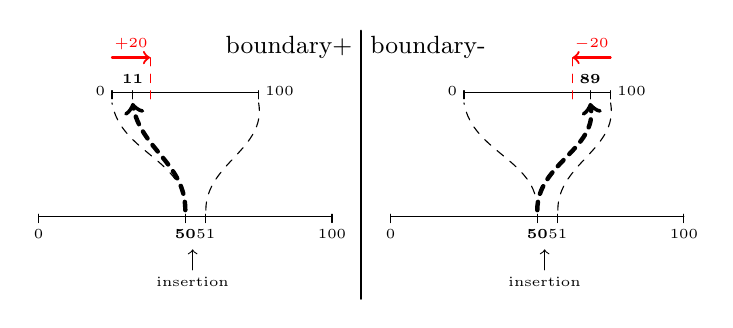
\begin{tikzpicture}[scale=0.745,cap=round]
\small

%% Titles
  \draw (5.5,82pt) -- node[anchor=east]{boundary+} (5.5,82pt);
  \draw (5.5,82pt) -- node[anchor=west]{boundary-} (5.5,82pt);

\tiny
%% Boundary +
  \draw [<-] (2.625,-16pt)--( 2.625, -26pt)  node[anchor=north] {insertion};

  \draw  (1.25,60pt)-- ( 3.75, 60pt);
  \draw  (0,0)-- (5, 0);
  
  \draw [dashed] (2.5,3pt) to[out=90,in=280] (1.25,55pt);
  \draw [->,ultra thick,dashed] (2.5,3pt) to[out=90,in=280] (1.6,55pt);
  \draw [dashed] (2.85,3pt) to[out=90,in=280] (3.75,55pt);  
  
  \draw [->,thick,color=red] (1.25,77pt) -- node[anchor=south]{$+20$}
  (1.9,77pt);
  \draw [dashed, color=red] (1.9,77pt) -- (1.9,57pt);


  \draw (0,1pt) -- (0,-3pt) node[anchor=north] {0};
  \draw (5,1pt) -- (5,-3pt) node[anchor=north] {$100$};
  \draw (1.25,57pt) -- (1.25,61pt) node[anchor=east] {0};
  \draw (1.6,57pt) -- (1.6,61pt) node[anchor=south] {\textbf{11}};
  \draw (3.75,57pt) -- (3.75,61pt) node[anchor=west] {$100$};
  \draw (2.5,1pt) -- (2.5,-3pt) node[anchor=north] {\textbf{50}};
  \draw (2.85,1pt) -- (2.85,-3pt) node[anchor=north] {$51$};


%% Delimitation
  \draw [thick] (5.5,-40pt) -- (5.5, 90pt);

%% Boundary -
  \draw [<-] (8.625,-16pt)--( 8.625, -26pt)  node[anchor=north] {insertion};

  \draw  (7.25,60pt)-- ( 9.75, 60pt);
  \draw  (6,0)-- (11, 0);
  
  \draw [dashed] (8.5,3pt) to[out=90,in=280] (7.25,55pt);
  \draw [->,ultra thick,dashed] (8.5,3pt) to[out=90,in=280] (9.4,55pt);
  \draw [dashed] (8.85,3pt) to[out=90,in=280] (9.75,55pt);  

  \draw [->,thick,color=red] (9.75,77pt) -- node[anchor=south]{$-20$}
  (9.1,77pt);
  \draw [dashed, color=red] (9.1,77pt) -- (9.1,57pt);
  
  \draw (6,1pt) -- (6,-3pt) node[anchor=north] {0};
  \draw (11,1pt) -- (11,-3pt) node[anchor=north] {$100$};
  \draw (7.25,57pt) -- (7.25,61pt) node[anchor=east] {0};
  \draw (9.4,57pt) -- (9.4,61pt) node[anchor=south] {\textbf{89}};
  \draw (9.75,57pt) -- (9.75,61pt) node[anchor=west] {$100$};
  \draw (8.5,1pt) -- (8.5,-3pt) node[anchor=north] {\textbf{50}};
  \draw (8.85,1pt) -- (8.85,-3pt) node[anchor=north] {$51$};


\end{tikzpicture}


\caption{Choice of the digit part of identifiers in \emph{boundary+} (left) and
  \emph{boundary-} (right). In both cases: constant base is set to $100$,
  boundary value is set to $20$ and the random number is $11$. The results are
  $[50.11]$ (\emph{boundary+}) and $[50.89]$ (\emph{boundary-}).}
\label{img:positionchoice}
\end{center}
\end{figure}

As expected, while the \emph{boundary+} algorithm handles the end editing,
the \emph{boundary--} algorithm aims the front editing. They both have
an antagonist weakness. Thus, \emph{boundary--} cannot be used alone safely,
just like \emph{boundary+}.

\subsection{Strategy choice}

Current variable-size sequence CRDTs rely on a unique strategy that is not
versatile in the sense that it does not adapt to every editing behaviour. As it
is impossible to know \emph{a priori} the editing behaviour and then, obtain
the best strategy for every sequence, \NAME{} randomly alternates between
\emph{boundary+} and \emph{boundary--}. Thus, when \NAME{} increases the
identifier size, it has $1\over{2}$ chance to choose either \emph{boundary+} or
\emph{boundary--}. This kind of choice implies lost depths but the main idea
is: some depths are lost indeed, nevertheless it is acceptable if the reward
compensates the losses.

%%%%%%% CHOOSE THE POSITION IN DENSE SPACE MANG %%%%%%%%
\begin{algorithm}[h]
\small
\algrenewcommand{\algorithmiccomment}[1]{\hskip2em$\rhd$ #1}

  \begin{algorithmic}[1]
  \State \textbf{let} $boundary := 10;$ \Comment{Any constant} 
  \State \textbf{let} $\mathcal{S} := \{\}$; 
  \Comment{map<depth,boolean>}
  \State \Comment{$true$: $boundary+$} 
  \State \Comment{$false$: $boundary-$} 
  \State

    \Function{alloc}{p, q $\in \mathcal{I}$}
    
      \State \textbf{let} $depth := 0$;
      \State \textbf{let} $interval := 0$;

      \While{$(interval < 1)$} \Comment{Not enough for 1 insert}
        \State $depth++$;
        \State $interval := prefix(q,depth) - prefix(p,depth) -1$;
      \EndWhile
      \State \textbf{let} $ste p:= min(boundary,interval)$; \Comment{Process 
        the maximum step to stay between $p$ and $q$}
      \State

      \If{$not(\mathcal{S}.exist(depth))$} \Comment{add the new entry}
        \State \textbf{let} $rand := RandBool()$;
        \State  $\mathcal{S}.set(depth, rand)$;
      \EndIf

      \If{$\mathcal{S}.get(depth)$} \Comment{$boundary+$}
        \State \textbf{let} $addVal := RandInt(0,step)+1$;
        \State \textbf{let} $id := prefix(p,depth) + addVal$;
      \Else \Comment{$boundary-$}
        \State \textbf{let} $subVal := RandInt(0,step)+1$;
        \State \textbf{let} $id := prefix(q,depth) - subVal$;
      \EndIf

      \State \textbf{return} $id$;
    \EndFunction
    
    \State

    \Function{prefix}{id $\in \mathcal{I}$, depth $\in \mathbb{N}^*$}
      \State \textbf{let} $idCopy := [\ ]$;
      \For{($cpt:=1$ to $depth$)}
        \If{($cpt<id.size$)} \Comment{Copy the value}
          \State $idCopy = idCopy.append(id.at(cpt))$;
          \Else \Comment{Add 0 encoded in the right base}
          \State $idCopy = idCopy.append(0_{base(cpt)})$; \label{line:base}
        \EndIf
      \EndFor
      \State \Return $idCopy$;
    \EndFunction

  \end{algorithmic}
\caption{\NAME{} allocation function}
\label{algo:strategychoicerandom}

\end{algorithm}


Algorithm~\ref{algo:strategychoicerandom} details the allocation function
\NAME{}. The departure base is set to $2^4$ (depth-0) and the \emph{boundary}
to $10$. The collection $\mathcal{S}$ stores the strategy choices. It starts
empty. Three parts compose the algorithm.
\begin{inparaenum}[(1)]
\item The first part processes the interval between the two identifiers $p$ and
  $q$ at each depth until one identifier at least can be inserted. The step
  limits the interval where $alloc$ will allocate the new identifier.
  \item The second part determines the allocation strategy. If the function did
    not allocate any identifiers at this depth yet, it randomly chooses among
    \emph{boundary+} and \emph{boundary--}. Then it saves this choice for
    future decisions in $\mathcal{S}$.
  \item The final part of the algorithm constructs the new
    identifier. Depending on the strategy, it draws a random value using the
    $step$ previously processed, and adds/subtracts this value to the $prefix$
    of $p$/$q$ at the wanted depth. The $prefix$ function takes an identifier
    $id$ as argument, and copies it until it reaches $depth$. If the identifier
    size is smaller than the requested depth, the function appends a zero to
    the copy for each missing depth. Each number in the sequence that composes
    the identifier must be carefully encoded in the base depending on the
    depth. Line~\ref{line:base} refers to $base(cpt)$. It is a very simple
    function that computes the base value at a given depth ($cpt$). Thus,
    $0_{base(cpt)}$ means that the binary representation of $0$ uses
    $log_2(base(cpt))$ bits. Consequently, the add and subtract operations do
    not require additional computation compared to regular arithmetic
    operations.
\end{inparaenum}

Figure~\ref{fig:lseqtreeexample} illustrates the allocation strategy \NAME{} by
showing its underlying tree model. First the empty sequence contains only two
identifiers: the beginning ($[0]$) and the end ($[31]$). The sequence needs
three additional identifiers between $[0]$ and $[31]$. First, \NAME{} randomly
assigns \emph{boundary+} as allocation strategy to the depth-1. Then, it
employs this strategy to allocate the three new identifiers ($[9]$, $[10]$,
$[23]$). The randomness makes the first and second elements very close in terms
of identifier distance.  Unfortunately, the sequence requests three other
identifiers between these two. Consequently, the depth has to grow to contain
these new elements. Since \NAME{} have not used any strategy at this depth yet,
it must randomly choose one. Here, the choice is \emph{boundary--}. Therefore,
this strategy allocates the three new identifiers. Furthermore, the underlying
exponential tree model extends the number of possible identifiers to $64$. In
this example, the resulting fresh identifiers are $[9.32]$, $[9.51]$ and
$[9.60]$.

\begin{figure}[h]
\addtolength{\belowcaptionskip}{-10pt}
\begin{center}
\begin{figure}[h]
\begin{center}

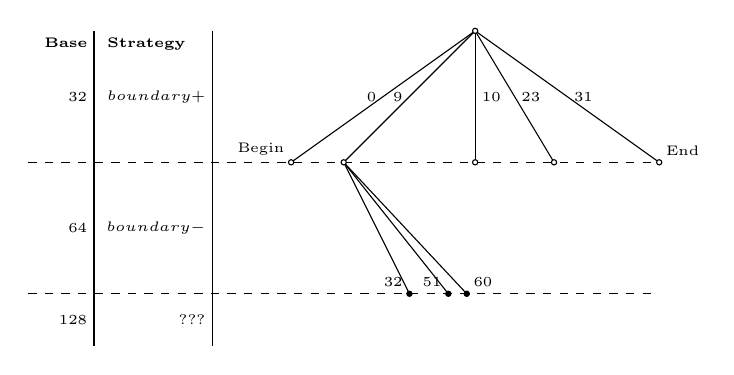
\begin{tikzpicture}[scale=0.95]
\tiny

  \draw (-100pt,0)node[anchor=north east]{\textbf{Strategy}\ \ \ \ }--
        (-100pt,-120pt);
  \draw (-145pt,0)node[anchor=north east]{\textbf{Base}\ }--
        (-145pt,-120pt);
  \draw (-100pt, -25pt) node[anchor=east]{$boundary+$} -- (-100pt, -25pt);
  \draw (-145pt, -25pt) node[anchor=east]{$32$} -- (-145pt, -25pt);
  \draw (-100pt, -75pt) node[anchor=east]{$boundary-$} -- (-100pt, -75pt);
  \draw (-145pt, -75pt) node[anchor=east]{$64$} -- (-145pt, -75pt);
  \draw (-100pt,-110pt) node[anchor=east]{$???$} -- (-100pt,-110pt);
  \draw (-145pt,-110pt) node[anchor=east]{$128$} -- (-145pt,-110pt);
  \draw[dashed] (-170pt,- 50pt) -- (70pt,- 50pt);
  \draw[dashed] (-170pt,-100pt) -- (70pt,-100pt);


  \draw (0,0) -- node[anchor=east]{0}   (-70pt, -50pt);
  \draw (0,0) -- node[anchor=west]{31}  ( 70pt, -50pt);

  \draw (0,0) -- node[anchor=east]{9}  (-50pt, -50pt);
  \draw (0,0) -- node[anchor=west]{10} (  0pt, -50pt);
  \draw (0,0) -- node[anchor=west]{23} ( 30pt, -50pt);

  \draw (-50pt, -50pt) -- (-25.0pt, -100pt);
  \draw (-50pt, -50pt) -- (-10.2pt, -100pt);
  \draw (-50pt, -50pt) -- (- 3.2pt, -100pt);

  \draw[fill=white] (0,0) circle (1pt);

  \draw[fill=white] (-70pt, -50pt) node[anchor=south east]{Begin} circle (1pt);
  \draw[fill=white] ( 70pt, -50pt) node[anchor=south west]{End} circle (1pt);

  \draw[fill=white] (-50pt, -50pt) circle (1pt);
  \draw[fill=white] (  0pt, -50pt) circle (1pt);
  \draw[fill=white] ( 30pt, -50pt) circle (1pt);

  
  \filldraw[black] (-25.0pt, -100pt) node[anchor=south east]{32} circle (1pt);
  \filldraw[black] (-10.2pt, -100pt) node[anchor=south east]{51} circle (1pt);
  \filldraw[black] (- 3.2pt, -100pt) node[anchor=south west]{60} circle (1pt);

\end{tikzpicture}
\caption{Underlying tree model of \NAME{} containing three identifiers at
  depth-1. The randomness makes the first and second element very close regard
  of identifiers ($[9]$ and $[10]$). The sequence requests three other elements
  between these two. The chosen strategy is \emph{boundary--} and since \NAME{}
  doubles the base at each depth, it allocates the fresh identifiers closer of
  $[10.64]$.}
\label{fig:lseqtreeexample}
\end{center}
\end{figure}

\caption{Underlying tree model of \NAME{} containing three identifiers at
  depth-1. The randomness makes the first and second elements very close
  regarding their identifiers ($[9]$ and $[10]$). The sequence requests three
  other elements between these two. The chosen strategy is \emph{boundary--}
  and since \NAME{} doubles the base at each depth, it allocates the fresh
  identifiers closer of $[10.64]$.}
\label{fig:lseqtreeexample}
\end{center}
\end{figure}

This example highlights the principle of \NAME{}.
Figure~\ref{fig:lseqtreeexample} depicts an exponential tree model that clearly
grows in arity over depths. It means more and more available identifiers when
the tree grows. This design aims to adjust the depth of the tree to the number
of insert operations. The next section aims to demonstrate experimentally that
\NAME{} achieves sub-linear space complexity in extreme setups and also
outperforms state-of-the-art CRDTs on real documents.

